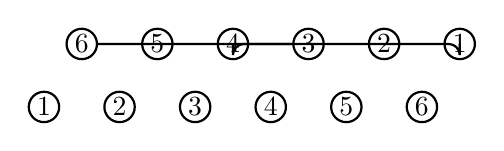
\begin{tikzpicture}[thick, scale=0.8, xscale=0.6]
	\def\numNodes{6}
	\pgfmathtruncatemacro{\numNodess}{\numNodes-1}
	\pgfmathtruncatemacro{\halfNodes}{\numNodes/2}
	\pgfmathtruncatemacro{\halfNodess}{\halfNodes-1}
	
	% Nodes (folded)
	\foreach \x in {1,...,\numNodes}{
		\ifthenelse{\x < \halfNodes \OR \x = \halfNodes}{
			\pgfmathtruncatemacro{\xx}{\x*2}
			\node (node \x) at (\xx,0)
			      [draw, circle, inner sep=0.1em]
			      {\x};
		}{
			\pgfmathtruncatemacro{\xx}{3 + \numNodes*2 - (\x*2)}
			\node (node \x) at (\xx,1)
			      [draw, circle, inner sep=0.1em]
			      {\x};
		}
	}
	
	% Wires between nodes
	\foreach \x in {1,...,\halfNodess}{
		\pgfmathtruncatemacro{\xx}{\x+1}
		\pgfmathtruncatemacro{\y}{\halfNodes + \x}
		\pgfmathtruncatemacro{\yy}{\y+1}
		\draw (node \x) -- (node \xx);
		\draw (node \y) -- (node \yy);
	}
	
	% End-wires
	\foreach \x in {\halfNodes, \numNodes}{
		\pgfmathtruncatemacro{\xx}{Mod(\x,\numNodes)+1}
		\draw [rounded corners] (node \x) -| (node \xx);
	}
\end{tikzpicture}

